\section{Vergleich der El. Masch}

\begin{longtable}{| p{.30\textwidth} | p{.60\textwidth} |}
    \hline
    
    \textbf{Aufbau}&
     \newline
    \tabbild[scale=0.55]{images/VergleichMotor}
    \\ \hline
    
    \textbf{Komplexität des Aufbaus}&
     \newline
    \tabbild[scale=0.5]{images/VergleichMotorKomplex}
    \\ \hline
    
    \textbf{Kosten}&
     \newline
    \tabbild[scale=0.5]{images/VergleichMotorKosten}
    \\ \hline
    
    \textbf{Wirkungsgrad}&
     \newline
    \tabbild[scale=0.5]{images/VergleichMotorWirkungsgrad}
    \\ \hline
    
    \textbf{Anpassungsfähigkeit}&
     \newline
    \tabbild[scale=0.5]{images/VergleichMotorAnpassung}
    \\ \hline
    
    \textbf{Anlaufstrom}&
     \newline
    \tabbild[scale=0.5]{images/VergleichMotorAnlaufstrom}
    \\ \hline
    
    \textbf{Anlaufmoment}&
     \newline
    \tabbild[scale=0.5]{images/VergleichMotorAnlaufmoment}
    \\ \hline
    
    \textbf{Drehzahlregelung}&
     \newline
    \tabbild[scale=0.5]{images/VergleichMotorDrehzahl}
    \\ \hline
    
    \textbf{Anwendungsbereich}&
     \newline
    \tabbild[scale=0.5]{images/VergleichMotorAnwendung}
    \\ \hline   
\end{longtable}   
\clearpage
\pagebreak
\subsection{Auswahl Flowchart}

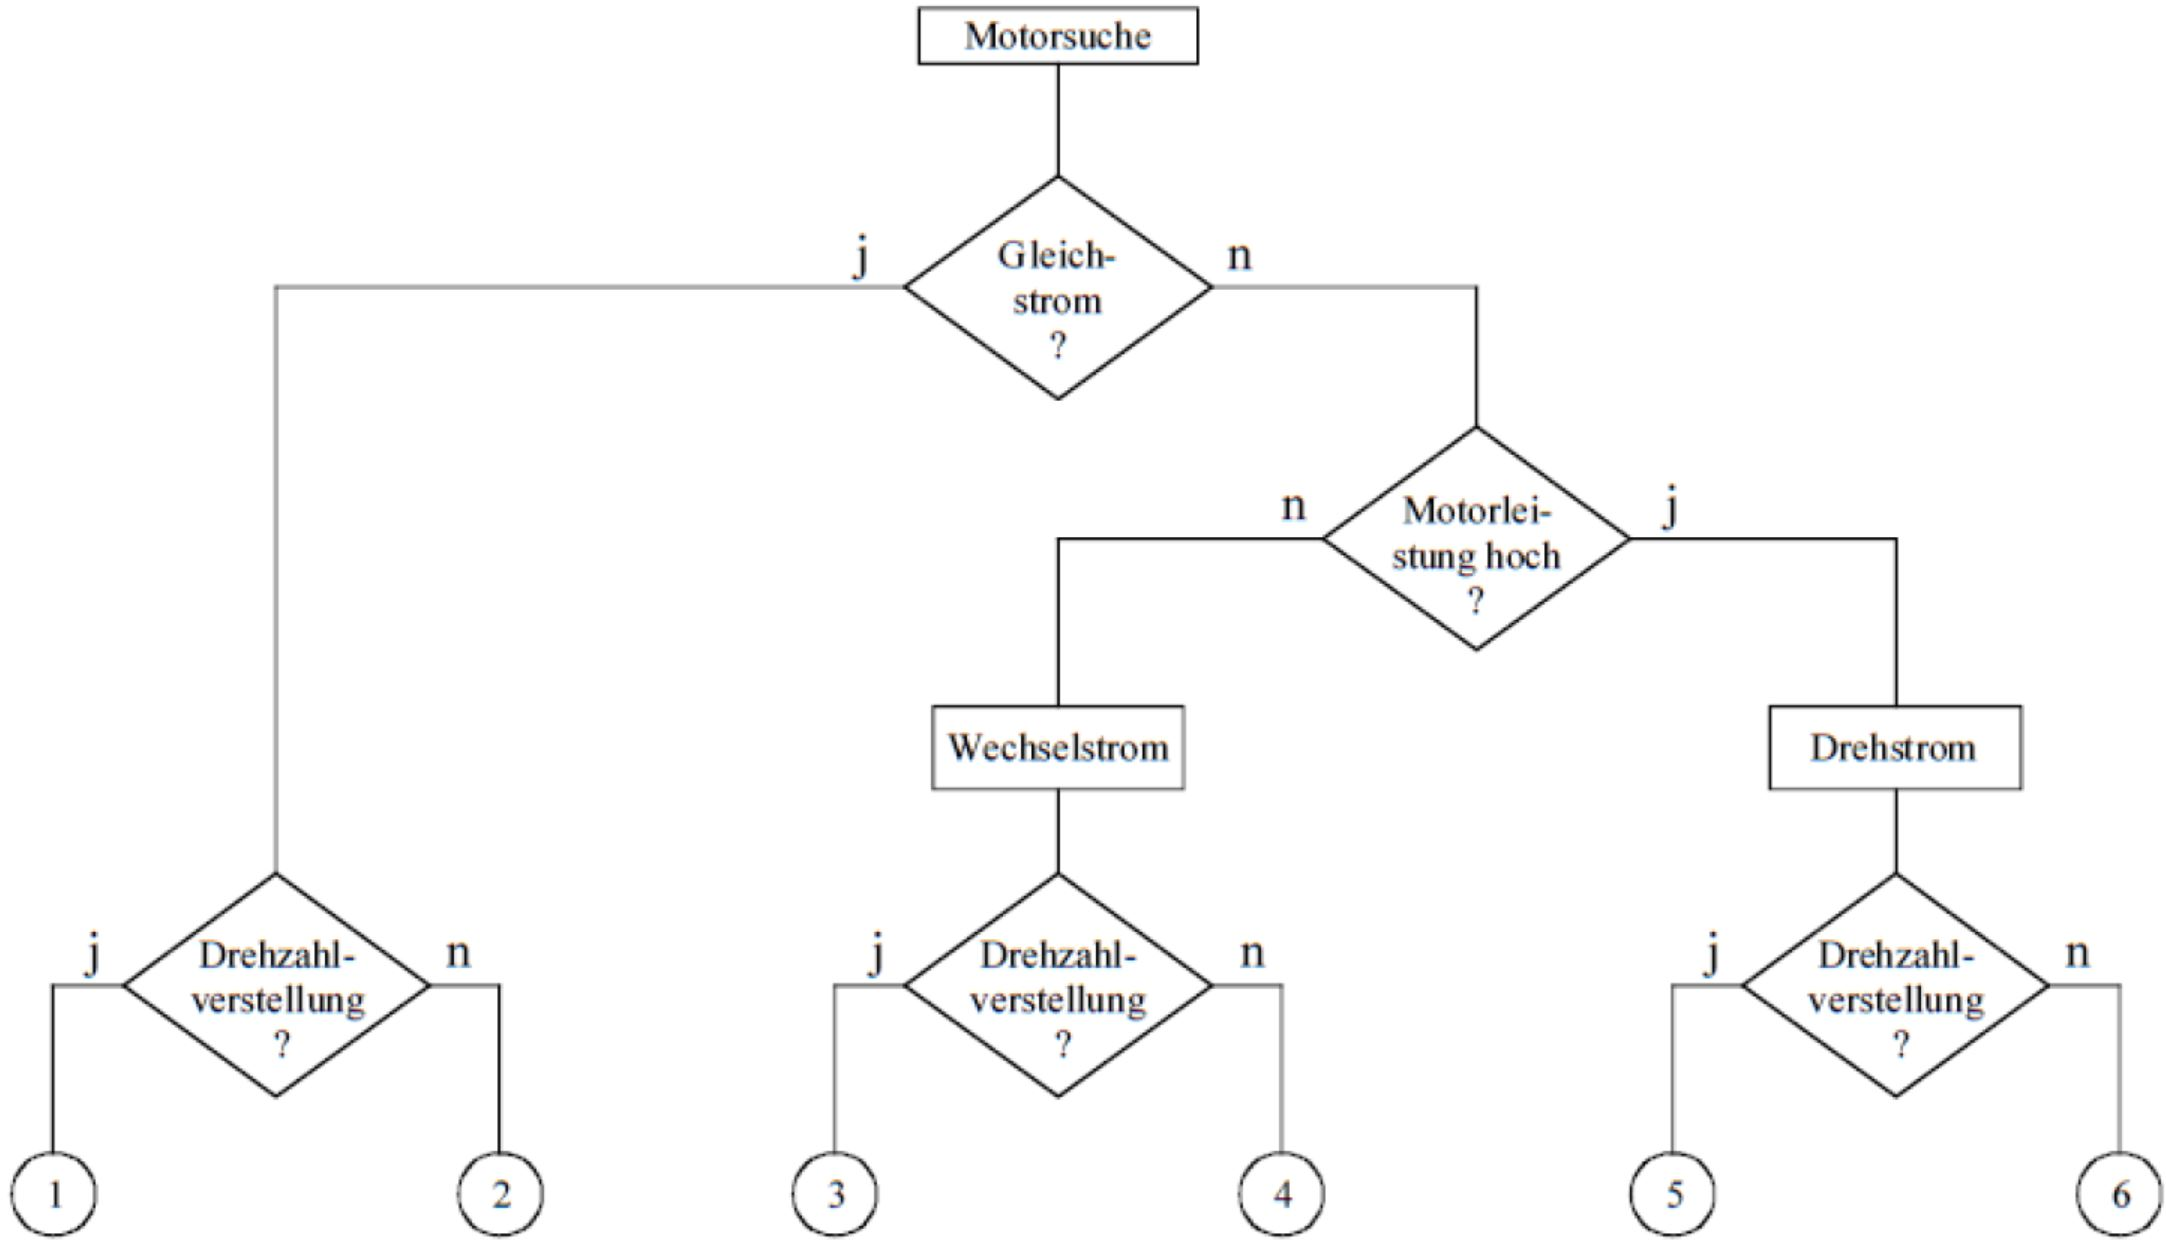
\includegraphics[scale=1]{images/Motorauswahl}
\\
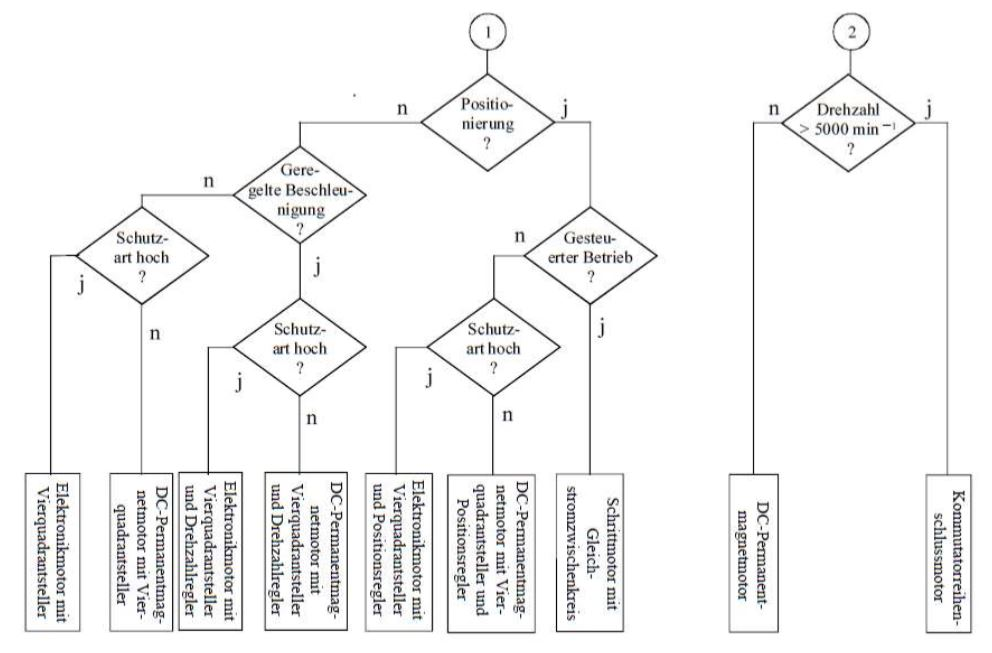
\includegraphics[scale=1]{images/Motorauswahl2}
\\
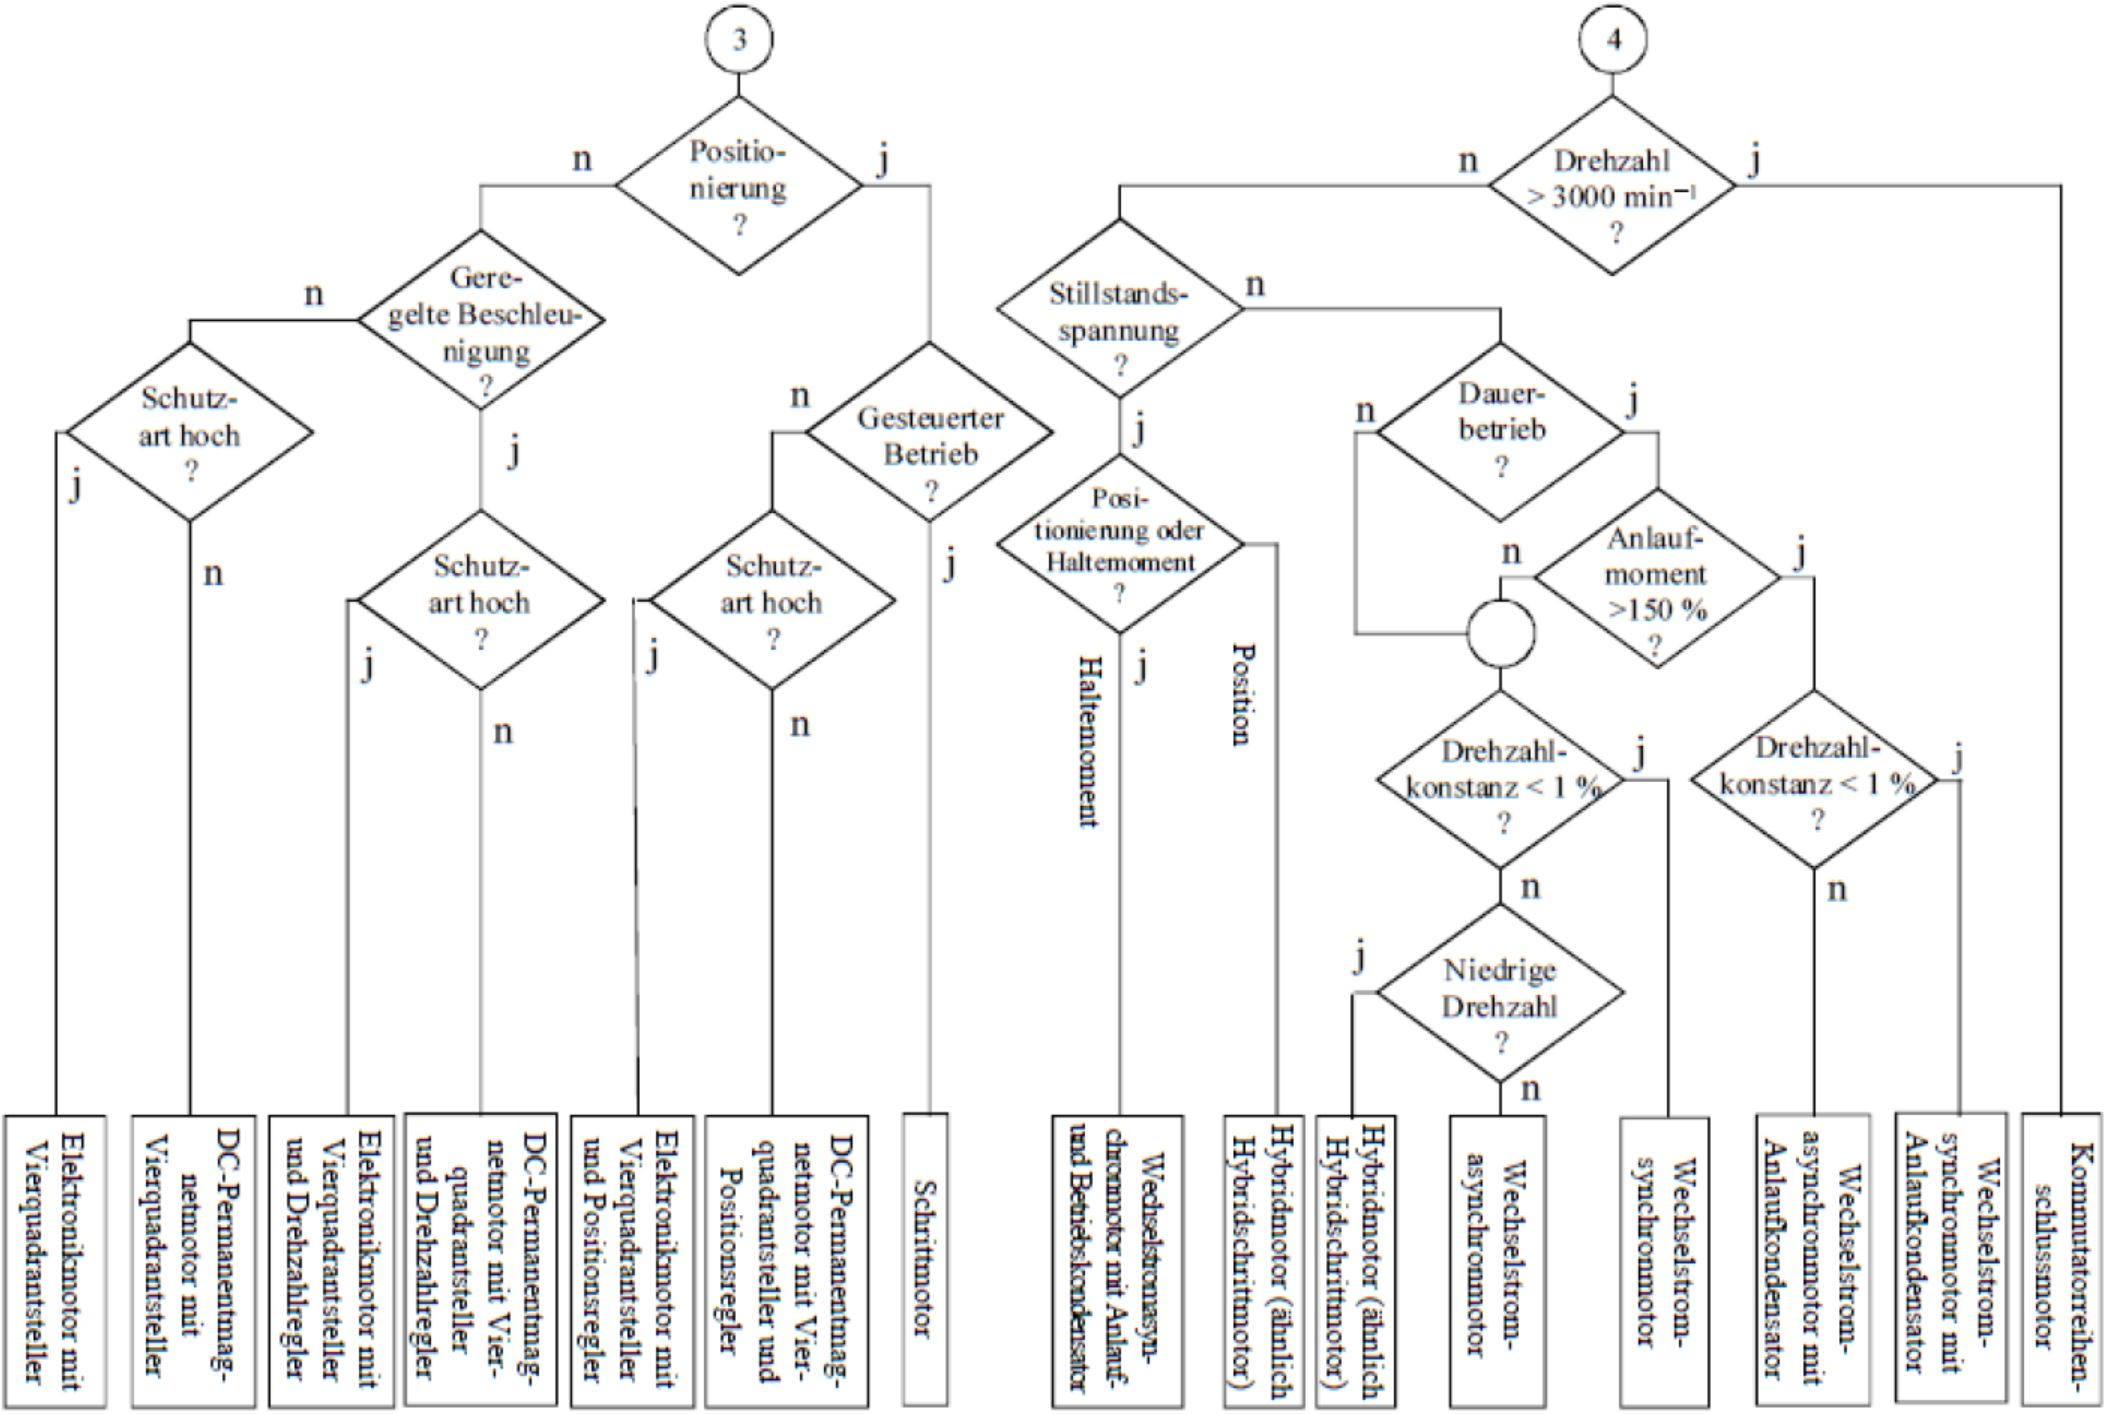
\includegraphics[scale=1]{images/Motorauswahl3}
\\
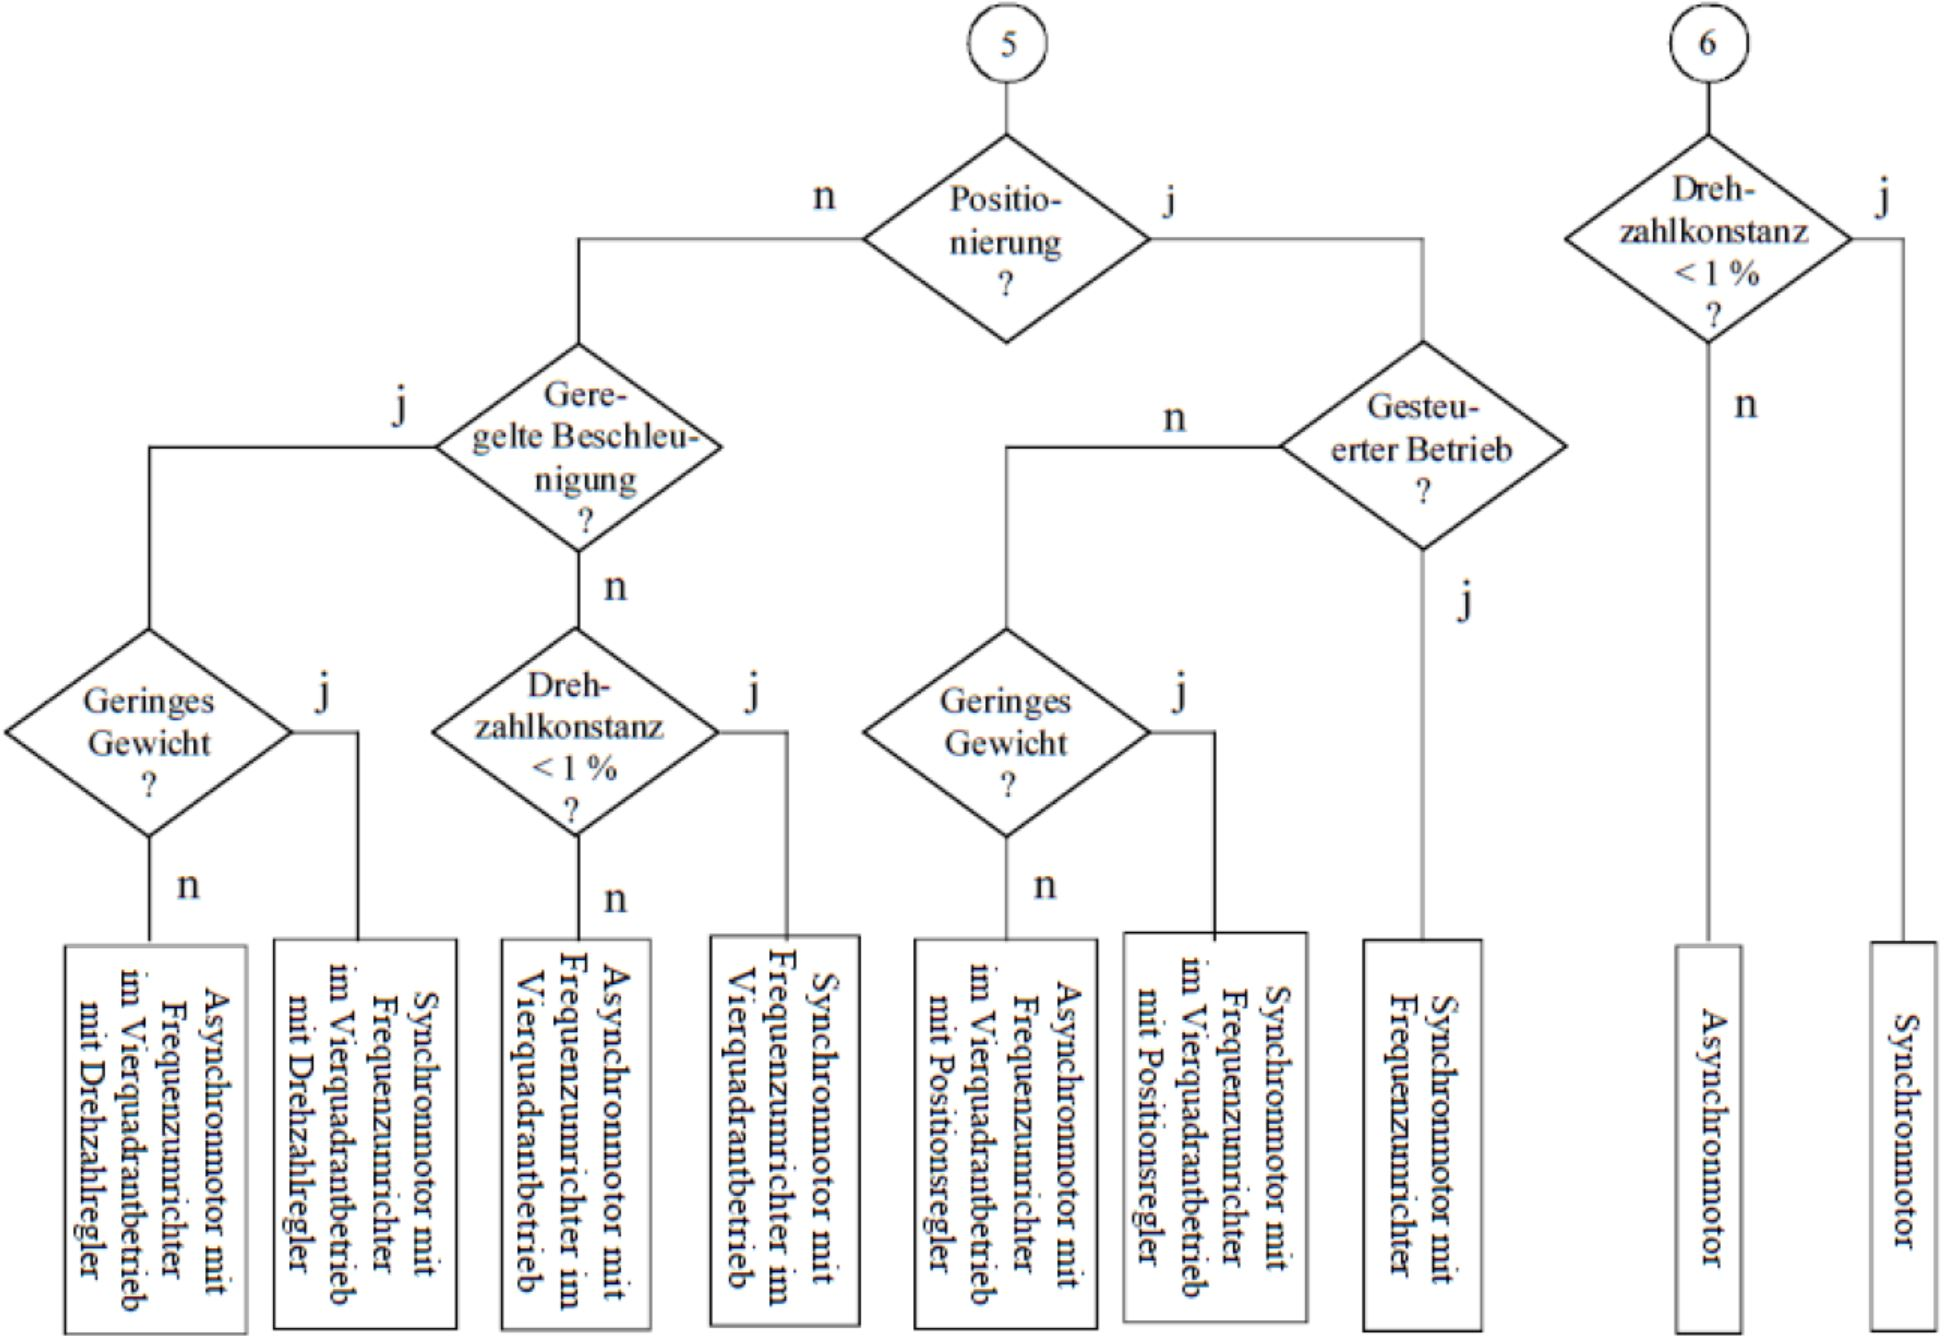
\includegraphics[scale=1]{images/Motorauswahl4}
\clearpage